\definecolor{vgray}{HTML}{CFCFCF}
\definecolor{vzero}{HTML}{DDF3DE}
\definecolor{va1}{HTML}{F4F4F4}
\definecolor{va2}{HTML}{F5E5E3}
\definecolor{va3}{HTML}{F5F1F1}
\definecolor{va4}{HTML}{E6F3E7}
\definecolor{va5}{HTML}{DFF3E0}
\definecolor{va6}{HTML}{E0F3E1}
\definecolor{va7}{HTML}{EDF4ED}
\definecolor{va9}{HTML}{E2F3E3}
\definecolor{va10}{HTML}{C25D5C}
\definecolor{vb1}{HTML}{F5D9D6}
\definecolor{vb6}{HTML}{F0F4F0}
\definecolor{vb7}{HTML}{F1F4F1}
\definecolor{vb9}{HTML}{E3F3E4}
\definecolor{vb10}{HTML}{CF7B78}
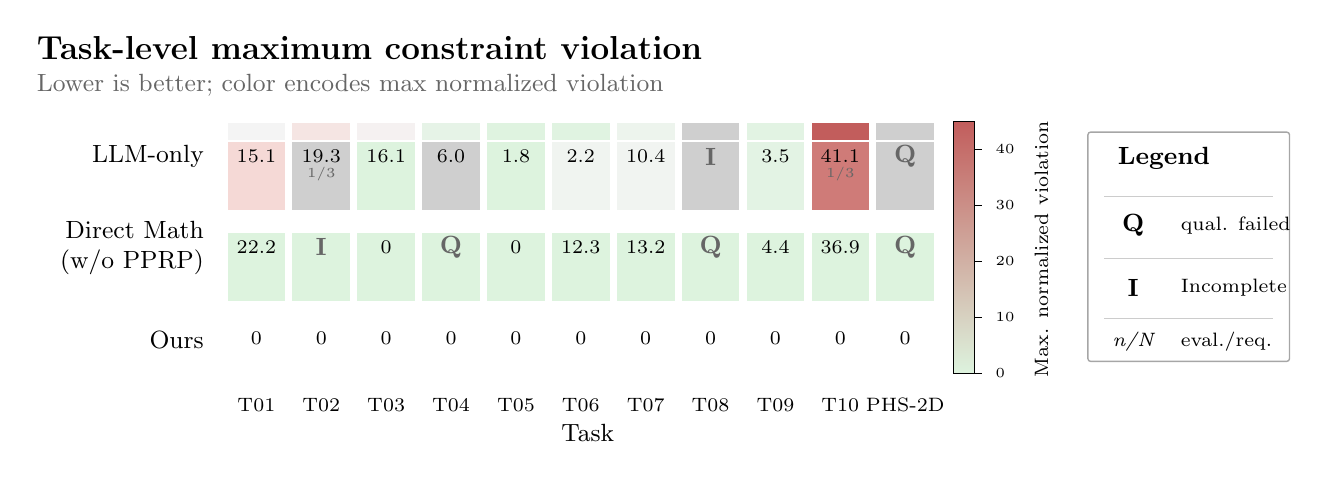
\begin{tikzpicture}[x=1.60cm,y=1.25cm,font=\sffamily]
% Heading
\node[anchor=west,font=\bfseries\large] at (0,3.28) {Task-level maximum constraint violation};
\node[anchor=west,font=\small,text=black!60] at (0,2.91) {Lower is better; color encodes max normalized violation};

% Method labels
\node[anchor=east,align=right,font=\small] at (1.48,2.18) {LLM-only};
\node[anchor=east,align=right,font=\small] at (1.48,1.25) {Direct Math\\(w/o PPRP)};
\node[anchor=east,align=right,font=\small] at (1.48,0.32) {Ours};

% Cell geometry
\def\xzero{1.58}
\def\cw{0.48}
\def\cg{0.035}
\def\ch{0.72}
\def\ytop{2.54}
\foreach \j/\task in {0/T01,1/T02,2/T03,3/T04,4/T05,5/T06,6/T07,7/T08,8/T09,9/T10,10/PHS-2D}{
  \pgfmathsetmacro{\xx}{\xzero+\j*(\cw+\cg)}
  \node[font=\scriptsize,anchor=north] at (\xx+\cw/2,-0.18) {\task};
}
% A: LLM-only
\foreach \j/\col in {0/va1,1/va2,2/va3,3/va4,4/va5,5/va6,6/va7,7/vgray,8/va9,9/va10,10/vgray}{
  \pgfmathsetmacro{\xx}{\xzero+\j*(\cw+\cg)}
  \path[fill=\col,draw=white,line width=1pt] (\xx,\ytop-\ch) rectangle ++(\cw,\ch);
}
% B: Direct Math
\foreach \j/\col in {0/vb1,1/vgray,2/vzero,3/vgray,4/vzero,5/vb6,6/vb7,7/vgray,8/vb9,9/vb10,10/vgray}{
  \pgfmathsetmacro{\xx}{\xzero+\j*(\cw+\cg)}
  \path[fill=\col,draw=white,line width=1pt] (\xx,\ytop-\ch-0.20) rectangle ++(\cw,\ch);
}
% C: Ours
\foreach \j in {0,...,10}{
  \pgfmathsetmacro{\xx}{\xzero+\j*(\cw+\cg)}
  \path[fill=vzero,draw=white,line width=1pt] (\xx,\ytop-2*\ch-0.40) rectangle ++(\cw,\ch);
}
% Cell values
\def\celltext#1#2#3#4{\node[font=\scriptsize,align=center,text=#4] at (#1,#2) {#3};}
\foreach \j/\val in {0/15.1,1/19.3,2/16.1,3/6.0,4/1.8,5/2.2,6/10.4,8/3.5,9/41.1}{
  \pgfmathsetmacro{\xx}{\xzero+\j*(\cw+\cg)+\cw/2}
  \celltext{\xx}{\ytop-\ch/2}{\val}{black}
}
\foreach \j in {1,9}{
  \pgfmathsetmacro{\xx}{\xzero+\j*(\cw+\cg)+\cw/2}
  \node[font=\tiny,text=black!60] at (\xx,\ytop-0.54) {1/3};
}
\pgfmathsetmacro{\xEight}{\xzero+7*(\cw+\cg)+\cw/2}
\pgfmathsetmacro{\xTen}{\xzero+10*(\cw+\cg)+\cw/2}
\node[font=\small\bfseries,text=black!60] at (\xEight,\ytop-\ch/2) {I};
\node[font=\small\bfseries,text=black!60] at (\xTen,\ytop-\ch/2) {Q};

\foreach \j/\val in {0/22.2,5/12.3,6/13.2,8/4.4,9/36.9}{
  \pgfmathsetmacro{\xx}{\xzero+\j*(\cw+\cg)+\cw/2}
  \node[font=\scriptsize] at (\xx,\ytop-\ch-0.20-\ch/2) {\val};
}
\foreach \j in {2,4}{
  \pgfmathsetmacro{\xx}{\xzero+\j*(\cw+\cg)+\cw/2}
  \node[font=\scriptsize] at (\xx,\ytop-\ch-0.20-\ch/2) {0};
}
\foreach \j in {1}{
  \pgfmathsetmacro{\xx}{\xzero+\j*(\cw+\cg)+\cw/2}
  \node[font=\small\bfseries,text=black!60] at (\xx,\ytop-\ch-0.20-\ch/2) {I};
}
\foreach \j in {3,7,10}{
  \pgfmathsetmacro{\xx}{\xzero+\j*(\cw+\cg)+\cw/2}
  \node[font=\small\bfseries,text=black!60] at (\xx,\ytop-\ch-0.20-\ch/2) {Q};
}

\foreach \j in {0,...,10}{
  \pgfmathsetmacro{\xx}{\xzero+\j*(\cw+\cg)+\cw/2}
  \node[font=\scriptsize] at (\xx,\ytop-2*\ch-0.40-\ch/2) {0};
}
% Axis label
\node[font=\small] at (4.45,-0.63) {Task};

% Color scale
\shade[shading=axis,bottom color=vzero,color=white,top color=va10] (7.35,-0.02) rectangle (7.52,2.54);
\draw[black,line width=0.4pt] (7.35,-0.02) rectangle (7.52,2.54);
\foreach \v in {0,10,20,30,40}{
  \pgfmathsetmacro{\yy}{-0.02+\v/45*2.56}
  \draw[line width=0.35pt] (7.52,\yy) -- (7.58,\yy);
  \node[anchor=west,font=\tiny] at (7.61,\yy) {\v};
}
\node[rotate=90,font=\scriptsize] at (8.05,1.24) {Max. normalized violation};

% Compact legend
\draw[rounded corners=1pt,draw=black!35,line width=0.5pt] (8.42,0.10) rectangle (10.02,2.43);
\node[anchor=west,font=\small\bfseries] at (8.58,2.16) {Legend};
\draw[black!20,line width=0.35pt] (8.55,1.78) -- (9.89,1.78);
\node[font=\small\bfseries] at (8.78,1.48) {Q};
\node[anchor=west,font=\scriptsize] at (9.08,1.48) {qual. failed};
\draw[black!20,line width=0.35pt] (8.55,1.15) -- (9.89,1.15);
\node[font=\small\bfseries] at (8.78,0.85) {I};
\node[anchor=west,font=\scriptsize] at (9.08,0.85) {Incomplete};
\draw[black!20,line width=0.35pt] (8.55,0.54) -- (9.89,0.54);
\node[font=\scriptsize\itshape] at (8.78,0.30) {n/N};
\node[anchor=west,font=\scriptsize] at (9.08,0.30) {eval./req.};
\end{tikzpicture}
